\documentclass[fontset=founder]{ucedubook}
\noprintanswers

\usepackage{tabularray}

\pagestyle{chapter}

\graphicspath{{figures}}

\ctexset{
  section = {
    number = \chinese{section},
    name = {,、}
  }
}

\let\oldpi=\pi
\let\pi=\PI

\usepackage{esvect}
\let\oldvec=\vec
\let\vec=\vv



\begin{document}

\chapter*{2022年北京卷数学试题}

\section{单选题}

\begin{ti}[.16]
  已知全集$U=\Set{x|-3<x<3}$,集合$A=\Set{x|-2<x\le 1}$,则$\complement_U A=$(\qquad)。

  \begin{choices}
    \item $\left(-2,1\right]$
    \item $\left(-3,2\right)\cup\left[1,3\right)$
    \item $\left[-2,1\right)$
    \item $\left(-3,-2\right]\cup\left(1,3\right)$
  \end{choices}
\end{ti}


\begin{ti}[.16]
  若复数$z$满足$\mathrm{i}\cdot z=3-4\mathrm{i}$,则$z=$(\qquad)。

  \begin{choices}
    \item $1$
    \item $5$
    \item $7$
    \item $25$
  \end{choices}
\end{ti}


\begin{ti}[.16]
  若$2x+y-1=0$是圆$(x-a)^2+y^2=1$的一条对称轴,则$a=$(\qquad)。

  \begin{choices}
    \item $\frac{1}{2}$
    \item $-\frac{1}{2}$
    \item $1$
    \item $-1$
  \end{choices}
\end{ti}


\begin{ti}[.16]
  已知函数$f(x)=\frac{1}{1+2^x}$,则对任意实数$x$,有(\qquad)。

  \begin{choices}
    \item $f(-x)+f(x)=0$
    \item $f(-x)-f(x)=0$
    \item $f(-x)+f(x)=1$
    \item $f(-x)-f(x)=\frac{1}{3}$
  \end{choices}
\end{ti}


\begin{ti}[.16]
  已知函数$f(x)=\cos^2 x-\sin^2 x$,则(\qquad)。

  \begin{choices}
    \item $f(x)$在$\left(-\frac{\pi}{2},\frac{\pi}{2}\right)$上单调递减
    \item $f(x)$在$\left(-\frac{\pi}{4},\frac{\pi}{12}\right)$上单调递增
    \item $f(x)$在$\left(0,\frac{\pi}{3}\right)$上单调递减
    \item $f(x)$在$\left(\frac{\pi}{4},\frac{7\pi}{12}\right)$上单调递增
  \end{choices}
\end{ti}


\begin{ti}[.16]
  设$\{a_n\}$是公差不为$0$的无穷等差数列,则“$\{a_n\}$为递增数列”是“存在正整数$N_0$,当$n>N_0$时,$a_n>0$”的(\qquad)。

  \begin{choices}
    \item 充分而不必要条件
    \item 必要而不充分条件
    \item 充分必要条件
    \item 既不充分也不必要条件
  \end{choices}
\end{ti}


\begin{ti}[.25]
  在北京冬奥会上,国家速滑馆“冰丝带”使用高效环保的二氧化碳跨临界直冷制冰技术,为实现绿色冬奥作出了贡献。如图描述了一定条件下二氧化碳所处的状态与$T$和$\lg P$的关系,其中$T$表示温度,单位是$K$;$P$表示压强,单位是“$\mathrm{bar}$”。下列结论中正确的是(\qquad)。

  \hfill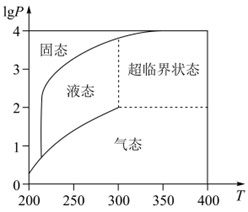
\includegraphics{北京-7.png}

  \begin{choices}
    \item 当$T=220$,$P=1026$时,二氧化碳处于液态
    \item 当$T=270$,$P=128$时,二氧化碳处于气态
    \item 当$T=300$,$P=9987$时,二氧化碳处于超临界状态
    \item 当$T=360$,$P=729$时,二氧化碳处于超临界状态
  \end{choices}
\end{ti}


\begin{ti}[.25]
  若$(2x-1)^4=a_4x^4+a_3x^3+a_2x^2+a_1x+a_0$,则$a_0+a_2+a_4=$(\qquad)。

  \begin{choices}
    \item $40$
    \item $41$
    \item $-40$
    \item $-41$
  \end{choices}
\end{ti}


\begin{ti}[.25]
  已知正三棱锥$P-ABC$的六条棱长均为$6$,$S$是$\triangle ABC$及其内部的点构成的集合。设集合$T=\Set{Q\in S|PQ\le 5}$,则$T$表示的区域面积为(\qquad)。

  \begin{choices}
    \item $\frac{3\pi}{4}$
    \item $\pi$
    \item $2\pi$
    \item $3\pi$
  \end{choices}
\end{ti}


\begin{ti}[.25]
  在$\triangle ABC$中,$AC=3$,$BC=4$,$\angle C=90^\circ$。$P$为$\triangle ABC$所在平面内的动点,且$PC=1$,则$\vec{PA}\cdot \vec{PB}$的取值范围是(\qquad)。

  \begin{choices}
    \item $\left[-5,3\right]$
    \item $\left[-3,5\right]$
    \item $\left[-6,4\right]$
    \item $\left[-4,6\right]$
  \end{choices}
\end{ti}


\newpageb
\section{填空题}

\begin{ti}[.2]
  函数$f(x)=\frac{1}{x}+\sqrt{1-x}$的定义域为\kong{}。
\end{ti}


\begin{ti}[.2]
  已知双曲线$y^2+\frac{x^2}{m}=1$的渐近线方程为$y=\pm \frac{\sqrt{3}}{3}x$,则$m=$\kong{}。
\end{ti}


\begin{ti}[.2]
  若函数$f(x)=A\sin x-\sqrt{3}\cos x$的一个零点为$\frac{\pi}{3}$,则$A=$\kong{};$f\left(\frac{\pi}{12}\right)=$\kong{}。
\end{ti}


\begin{ti}[.2]
  设函数 $f(x)=\begin{cases}
    -ax+1, & x<a \\
    (x-2)^2, & x\ge a
  \end{cases}$ ,若$f(x)$存在最小值,则$a$的一个取值为\kong{},$a$的最大值为\kong{}。
\end{ti}


\begin{ti}[.2]
  已知数列$\{a_n\}$各项均为正数,其前$n$项和$S_n$满足$a_n\cdot S_n=9$($n=1,2,\cdots$)。给出下列四个结论:

  \begin{choices}[0][4]
    \item $\{a_n\}$的第$2$项小于$3$;
    \item $\{a_n\}$为等比数列;
    \item $\{a_n\}$为递减数列;
    \item $\{a_n\}$中存在小于$\frac{1}{100}$的项。
  \end{choices}
  
  其中所有正确结论的序号是\kong{}。
\end{ti}


\newpageb
\section{解答题}

\begin{ti}
  在$\triangle ABC$中,$\sin 2C=\sqrt{3}\sin C$。

  (1)求$\angle C$;
  
  (2)若$b=6$,且$\triangle ABC$的面积为$6\sqrt{3}$,求$\triangle ABC$的周长。
\end{ti}


\begin{ti}
  如图,在三棱柱$ABC-A_1B_1C_1$中,侧面$BC C_1B_1$为正方形,平面$BC C_1B_1\perp$平面$AB B_1A_1$,$AB=BC=2$,$M$,$N$分别为$A_1B_1$,$AC$的中点。

  (1)求证:$MN\parallel $平面$ BC C_1B_1$;
  
  (2)再从条件①、条件②这两个条件中选择一个作为已知,求直线$AB$与平面$BMN$所成的角的正弦值。

  条件①:$AB\perp MN$;
  
  条件②:$BM=MN$。

  注:如果选择条件①和条件②分别解答,按第一个解答计分。

  \hfill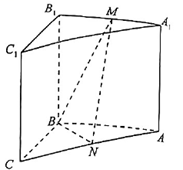
\includegraphics{北京-17.png}
\end{ti}


\newpageb

\begin{ti}
  在校运动会上,只有甲、乙、丙三名同学参加铅球比赛,比赛成绩达到$9.50\mathrm{\,m}$以上(含$9.50\mathrm{\,m}$)的同学将获得优秀奖。为预测获得优秀奖的人数及冠军得主,收集了甲、乙、丙以往的比赛成绩,并整理得到如下数据(单位:$\mathrm{m}$):

  甲:$9.80$,$9.70$,$9.55$,$9.54$,$9.48$,$9.42$,$9.40$,$9.35$,$9.30$,$9.25$;
  
  乙:$9.78$,$9.56$,$9.51$,$9.36$,$9.32$,$9.23$;
  
  丙:$9.85$,$9.65$,$9.20$,$9.16$。

  假设用频率估计概率,且甲、乙、丙的比赛成绩相互独立。

  (1)估计甲在校运动会铅球比赛中获得优秀奖的概率;

  (2)设$X$是甲、乙、丙在校运动会铅球比赛中获得优秀奖的总人数,估计$X$的数学期望$E(X)$;

  (3)在校运动会铅球比赛中,甲、乙、丙谁获得冠军的概率估计值最大?(结论不需要证明)
\end{ti}


\newpageb

\begin{ti}
  已知椭圆$E:\frac{x^2}{a^2}+\frac{y^2}{b^2}=1$($a>b>0$)的一个顶点为$A(0,1)$,焦距$2\sqrt{3}$。

  (1)求椭圆$E$的方程;

  (2)过点$P(-2,1)$作斜率为$k$的直线与椭圆$E$交于不同的两点$B$,$C$,直线$AB$,$AC$分别与$x$轴交于点$M$,$N$,当$\left|MN\right|=2$时,求$k$的值。
\end{ti}


\newpageb

\begin{ti}
  已知函数$f(x)=\mathrm{e}^{x}\ln (1+x)$。

  (1)求曲线$y=f(x)$在$(0,f(0))$处的切线方程;

  (2)设$g(x)=f'(x)$,讨论函数$g(x)$在$\left[0,+\infty\right)$上的单调性;

  (3)证明:对任意的$s,t\in \left(0,+\infty\right)$,有$f(s+t)>f(s)+f(t)$。
\end{ti}


\newpageb

\begin{ti}
  已知$Q:a_1,a_2,\cdots ,a_k$为有穷整数数列。给定正整数$m$,若对任意的$n\in \{1,2,\cdots ,m\}$,在$Q$中存在$a_i,a_{i+1},a_{i+2},\cdots ,a_{i+j}$($j\ge 0$),使得$a_i+a_{i+1}+a_{i+2}+\cdots +a_{i+j}=n$,则称$Q$为$m\:\!$--连续可表数列。

  (1)判断$Q:2,1,4$是否为$5\:\!$--连续可表数列?是否为$6\:\!$--连续可表数列?说明理由;

  (2)若$Q:a_1,a_2,\cdots ,a_k$为$8\:\!$--连续可表数列,求证:$k$的最小值为$4$;

  (3)若$Q:a_1,a_2,\cdots ,a_k$为$20\:\!$--连续可表数列,且$a_1+a_2+\cdots +a_k<20$,求证:$k\ge 7$。
\end{ti}



\end{document}